\newcommand{\chapterpepperapplication}{Kapitel 5. }

\chapter{Implementierung: Pepper App}
\label{sec:Pepper_Applikation}
\lhead{\chapterpepperapplication \emph{Implementierung der Pepper App}}


Nachdem die Einrichtung von Android Studio und die Planung der Hochschul-Anwendungen für Pepper abgeschlossen waren, ging es nun darum, unsere Anwendungsfälle zu implementieren. Der  erste Schritt war es, sich mit der Programmstruktur von Pepper vertraut zu machen. Da wir den  kompletten Code für die Touristik App der Masterstudenten als Referenz verwenden konnten, haben wir  uns schnell ein Bild von der Struktur machen können.\\

\section{Das Grundgerüst}
 
 (Abb. \ref{fig:FilesInAS}) Sobald ein neues Projekt in Android Studio erstellt wird, wird nachfolgende Ordner Struktur generiert.\\

\begin{figure}[H]
    \centering
    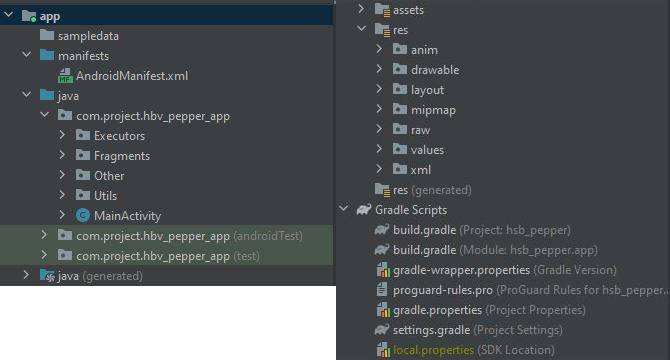
\includegraphics[width=13cm]{Figures/AppChapter/OrdnerStruktur.png}
    \caption{Grundgerüst Android Studio}
    \label{fig:FilesInAS}
    \centering
\end{figure}


\subsection*{/manifests}
In dem Ordner \verb|/manifests| befindet sich die konfigurations Datei \verb|AndroidManifest.xml|. In dieser Datei können verschiedene allgemeine Einstellungen zu Pepper getroffen werden. Die wichtigsten Einstellungen sind die \verb|permissions|. Dies sind Berechtigung-Parameter, mit denen bestimmte Komponenten von Pepper oder Verbindungen erlaubt werden können. Da wir im Code sehr oft Request an den Node-Server geschickt haben oder Webseiten auf dem Tablet von Pepper angezeigt haben, mussten wir zuerst die Verbindung mit dem Internet in der AndroidManifest erlauben. Auch das Zugreifen auf den Externen Speicher von Pepper kann in dieser Datei erlaubt und konfiguriert werden. Des Weiteren können alle wichtigen Pfade zu weiteren Config Dateien und der MainActivity Klasse gesetzt werden.

\subsection*{/java}
In  \verb|/java| befinden sich alle unsere Java Klassen und somit der komplette Code der Pepper Anwendung. Sobald ein neues Projekt in Android Studio erstellt wird, wird die MainActivity Klasse automatisch generiert. Diese Klasse ist auch das Herzstück von Pepper, da hier der komplette Code gestartet, gesteuert und beendet wird. Hierzu werden wir im späteren Verlauf mehr erzählen. Die Verzeichnisse, welche mit ``andoirdTest'' und ``test'' beschriben sind, werden für das Testen der Applikation verwendet. Diese haben wir in unserem Projekt nicht verwendet, daher gehen wir auf diesen Bereich nicht weiter ein.

\subsection*{/assets}
In \verb|/assets| können verschiedene Daten abgelegt werden, auf die im Code zu jeder Zeit zugegriffen werden kann. Zum Beispiel können JSON Dateien abgelegt und im Code gelesen und verändert werden.

\subsection*{/res}
In \verb|/res| finden sich die Ressourcen der Anwendung. Diese sind wie folgt gegliedert:

\subsubsection*{/res/Anim}
In dem ersten Unterordner \verb|/anim| befinden sich die Animationen von Pepper. Er besitzt die Möglichkeit, jedes Gelenk zu bewegen, um wie ein Mensch zu wirken. Die Pepper SDK besitzt eine eigene GUI, um Peppers Bewegungen zu konfigurieren und neue Animationen zu erstellen. In dem Editor befindet sich bereits eine große Auswahl an vordefinierten Bewegungen. In unsere Applikation haben wir bis auf die vordefinierte 
``idle Animation''  (Standardbewegung, wenn Pepper untätig ist) keine weiteren Animationen verwendet.

\subsubsection*{/res/drawable}
In dem \verb|/drawable| Ordner befinden sich alle Bilder, die auf dem Tablet angezeigt werden können.

\subsubsection*{/res/layout}
Der \verb|/layout| Ordner beinhaltet alle XML-Dateien, die für die Graphische Darstellung auf dem Tablet verwendet werden. Android 
Studio bietet hier ebenfalls eine GUI mit verschiedenen Komponenten zur Auswahl und eine Echtzeit Darstellung des Layouts.

\subsubsection*{/res/mipmap}
In \verb|/mipmap| (MIP = multum in parvo = vieles im Kleinen) befinden sich vorberechnete und optimierte Bildfolgen, die die Darstellungsqualität von Texturen verbessern, wenn diese kleiner als in der ursprünglichen Größe dargestellt werden. (vgl. Abb. \ref{fig:MipMap}) Dadurch, dass Texturen mithilfe der MipMaps verkleinert dargestellt werden, benötigt das Anzeigen von Bildern auf dem Tablet weniger Rechenzeit (mehr: \cite{MipMaps}).\\

\begin{figure}[H]
    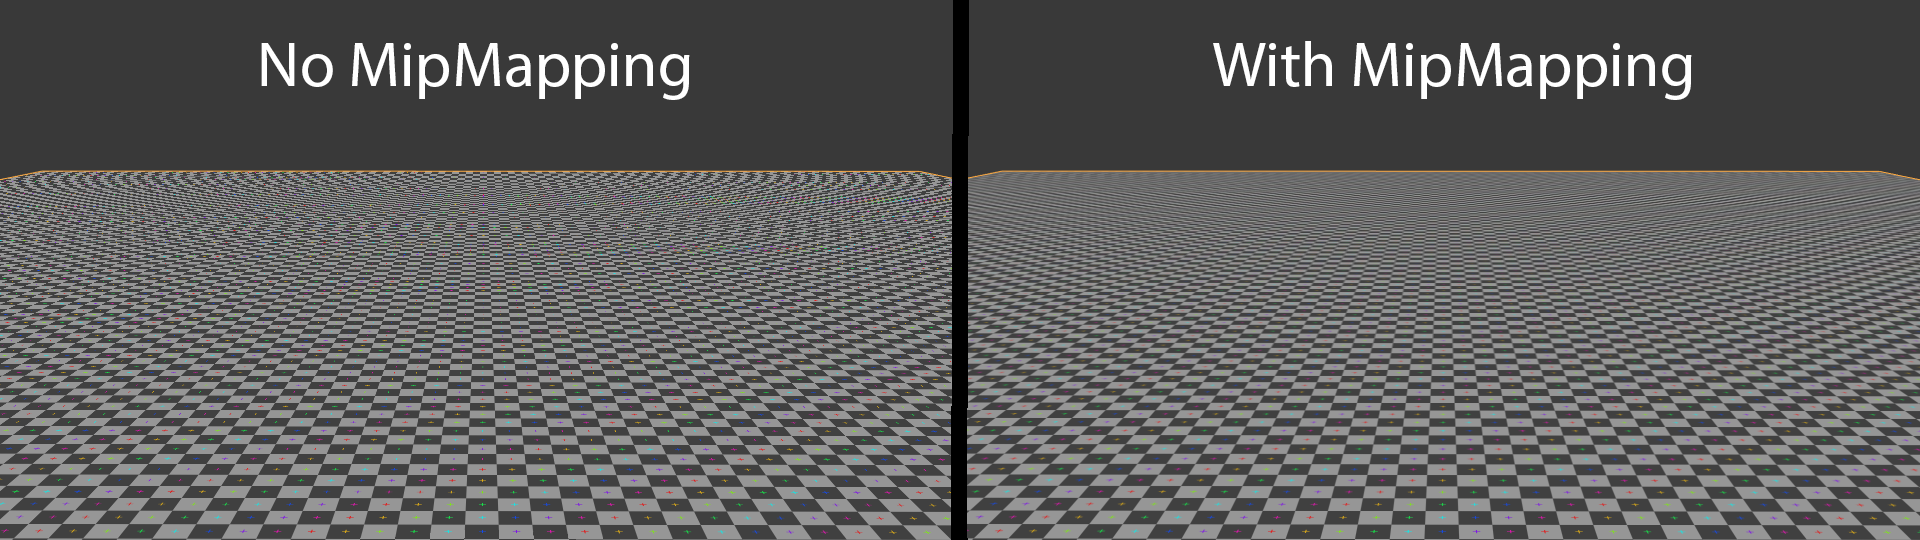
\includegraphics[width=\textwidth]{Figures/AppChapter/4_1_2.png}
    \caption{MipMapping \cite{mimappng}}
    \label{fig:MipMap}
    \centering
\end{figure}

\subsubsection*{/res/raw}
Der \verb|/raw| Ordner beinhaltet alle Topic Dateien der Anwendung und werden im Chatbot zur verbalen Interaktion mit dem Anwender verwendet. In den Topics können Gesprächsthemen vordefiniert und mit verschiedenen Funktionen verbunden werden. Die Syntax eines Topics ist relativ simpel gehalten und selbsterklärend, sodass es uns nicht schwer fiel, viele verschiedene Gesprächsthemen für unsere Anwendung zu entwickeln.

\subsubsection*{/res/values}
In \verb|/values| befinden sich alle XML-Dateien, die Werte für die verschiedenen Ressourcen bereitstellen. Dies sind zum Beispiel Werte wie Farben, Stilen oder Dimensionen.

\subsubsection*{/res/xml}
\verb|/xml| wurde manuell erstellt und beinhaltet hauptsächlich weitere XML-Dateien, die für Konfigurationen verwendet wurden. Hierauf werden wir im späteren Verlauf näher drauf eingehen. \\

\subsection*{gradle}
Im unteren Bereich befinden sich alle wichtigen Gradle Konfigurationsdateien. Gradle ist ein Build-Toolkit, um den Build-Prozess von Android Studio zu automatisieren und zu verwalten. Sobald der Code ausgeführt wird, werden zuerst alle Gradle Einstellungen ermittelt, Bibliotheken und Frameworks installiert und anschließend wird der Code kompiliert. Gradle erstellt anschließend eine APK (Android App Bundles), womit die Androidanwendung erstellt und gestartet werden kann. (Quelle: \cite{Gradle})
In der \verb|/build.gradle| Datei können benutzerdefinierte Build-Konfigurationen definiert werden. Hier kann zum Beispiel die Versionen der Pepper SDK verwaltet werden und außerdem können externe Frameworks, die nicht in der Standardbibliothek von Java enthalten sind, implementiert werden.\\

\section{Programmcode}

\subsection{MainActivity}

Die \verb|MainActivity| ist die Hauptklasse unserer Anwendung, da hier alle Prozesse gesteuert werden. Die Klasse wird mit der \verb|RobotActivity| Klasse erweitert, die mehrere Methoden bereitstellt, um das Verhalten von Pepper zu programmieren (vgl. Abb. \ref{fig:AAL}). Außerdem implementiert sie das \verb|RobotLifecycleCallbacks| Interface, die bestimmte Lebenszyklus-Methoden voraussetzt 
und bereitstellt. Diese können wie folgt zusammengefasst werden:\\

\begin{figure}[H]
    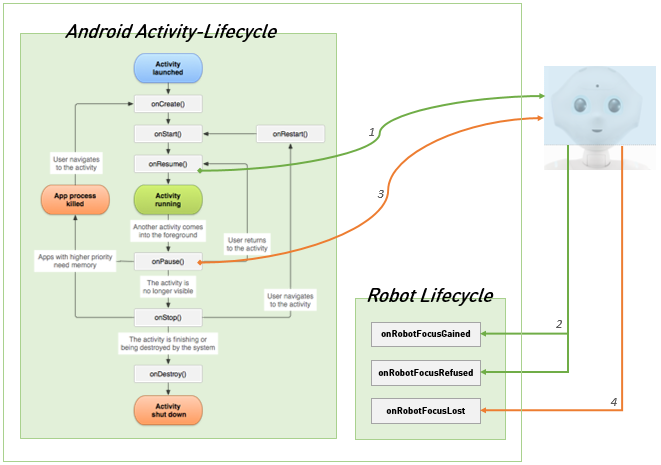
\includegraphics[width=\textwidth]{Figures/AppChapter/4_1_3.png}
    \caption{Android Activity-Lifecycle \cite{AALife}}
    \label{fig:AAL}
    \centering
\end{figure}

Die \textit{Android Activity Lifecycle} umfasst Methoden, welche in Android Studio als Standard bereitgestellt werden. Mit der qiSDK und deren \verb|RobotLifecycleCallbacks| kommen die \verb|Robot Lifecycle| Methoden hinzu, die speziell für Pepper entiwckelt worden sind. Alle diese Methoden werden automatisch aufgerufen, sobald Pepper einen bestimmten Punkt oder eine bestimmte Situation erreicht hat. (Dies sind Callback Methoden, welche auf bestimmte Events reagieren.)

Die komplette Applikation läuft auf einem Hauptprozess, der UI-Thread genannt wird. Die einzigen Ausnahmen, die nicht auf diesem Thread laufen, sind die Robot Lifecycle Methoden und natürlich auch asynchrone Funktionen.

Im Folgenden werden die wichtigsten \verb|Lifecycle-Methoden| erläutern:\\

\subsubsection{onCreate}

Die \verb|onCreate| Methode ist der erste Einstiegspunkt, sobald die Pepper Anwendung gestartet wird. Sie wird auch nur einmalig ausgeführt. Damit die Callbacks der RobotLifecycleCallbacks Implementation überhaupt funktioniert, ist der erste Schritt, das registrieren der QISDK. Des Weiteren haben wir in der \verb|onCreate| Methode alle erforderlichen Initialisierungen durchgeführt, wie zum Beispiel das Hinzufügen des Ressourcenordners oder die Spracheinstellung, die Pepper's Chatbot verwenden soll.
Mit \verb|setContentView| können wir bestimmen, was auf Pepper's Tablet angezeigt wird. Hier werden die XML-Dateien aus dem Layout Ordner geladen und in der ContentView initialisiert. \\

\subsubsection{onDestroy}

Die \verb|onDestroy| Methode wird ausgeführt, sobald die Anwendung beendet wird. Sie wird hauptsächlich dafür verwendet, um Ressourcen wie Threads freizugeben. In unserer Anwendung müssen wir hier zusätzlich die QISDK unregistriert, damit keine weiteren Lifecycle-Aufrufe auftreten. \\

\subsubsection{Focus Gained}

Die \verb|onRobotFocusGained| Methode ist ein Lifecycle exklusiv für Pepper. Diese wird aufgerufen, sobald Pepper eine Person im Fokus hat. Pepper richtet anschließend sein Kopf zu dieser Person und hält stets Blickkontakt. Selbst wenn die Person sich bewegt, verfolgt Pepper diese Person solange mit seinem Kopf, bis er den Fokus verliert. In dieser Methode werden alle Komponenten initialisiert, die zur Interaktion mit dem Anwender verwendet werden. Hierfür wird die Variable \verb|QiContext| übergeben, die es erlaubt, bestimmte Aktionen durchzuführen, Ressourcen bereitzustellen und verschiedene Dienste abzurufen. Hauptsächlich wird hier der Chatbot mithilfe des \verb|QiContext| bereitgestellt, sodass Pepper direkt mit dem Anwender verbal interagieren kann. Da der Chatbot stetig ausgeführt wird, während der Anwender mit Pepper spricht, wird dieser asynchron ausgeführt, um den Thread dieser Methode nicht zu unterbrechen. Zu dem Thema Chatbot werden wir im späteren Verlauf mehr erzählen. \\

\subsubsection{Focus Lost}
Sollte Pepper seinen Fokus zu dem Anwender verlieren, wird die \verb|onRobotFocusLost| Methode aufgerufen. Diese Methode wird hauptsächlich dazu verwendet, um die initialisierten Komponenten aus der \verb|onRobotFocusGained| Methode wieder zu beenden (Quelle: \cite{Robot_lifecycle}).\\

\subsection{Weitere Funktionen}

\subsubsection{Fragments}

Beim Entwickeln der Applikation haben wir die verschiedenen Pepper Projekte von Softbanks als Referenz verwendet. Diese bieten auf GitHub zahlreiche Beispielprojekte an, wie bestimmte Strukturen oder Funktionen implementiert werden. Eine Funktion, die wir als sehr hilfreich betrachtet haben, war das Aufteilen der Applikation in einzelne Fragmente. Hierbei haben wir uns an dem Template von softbankrobotics orientiert: \url{https://github.com/softbankrobotics-labs/App-Template}

Diese Fragmente besitzen ihre ganz eigenen Gesprächsthemen, Darstellungen und Funktionen. Der größte Vorteil an Fragmenten ist, dass die Topics voneinander getrennt werden können. Sollte eine Anwendung zum Beispiel sehr viele Topics besitzen, ist die Gefahr groß, dass Pepper etwas falsch versteht und eine Antwort zu einem anderen Gesprächsthema gibt.

Zu Beginn der Implementierung haben wir unser Projekt in drei verschiedene Fragmente aufgeteilt. Das Hauptmenü ist das erste Fragment, wo allgemeine Dinge gefragt werden können und mit Pepper Small Talk geführt werden kann (vgl. Abb. \ref{fig:Mainmenu}). Auf seinem Tablet haben wir ein Hauptmenü erstellt, wo per Knopfdruck das Fragment gewechselt werden kann. Der Anwender hat hier aber auch die öglichkeit, verbal das Fragment zu wechseln. Die anderen beiden Fragmente wurden anschließend getriggert, sobald danach gefragt oder der jeweilige Button gedrückt wurde. Das zweite Fragment beinhaltete alles rund um das Thema Hochschule und Bremerhaven. Hier konnte Pepper über alles ausgefragt werden, was mit diesen beiden Thema zutun hatte. In dem letzten Fragment waren unsere Anwendungsfälle implementiert. Sollte der Anwender sich den Stunden- oder Mensaplan anzeigen lassen wollen, so hätte er zuerst auf dieses Fragment wechseln müssen. Letztendlich haben wir unsere finale Applikation nicht in Fragmente aufgeteilt, sodass zu jeder Zeit nach jedem Thema gefragt werden konnte, ohne das Fragment wechseln zu müssen.\\

\begin{figure}[H]
    \centering
    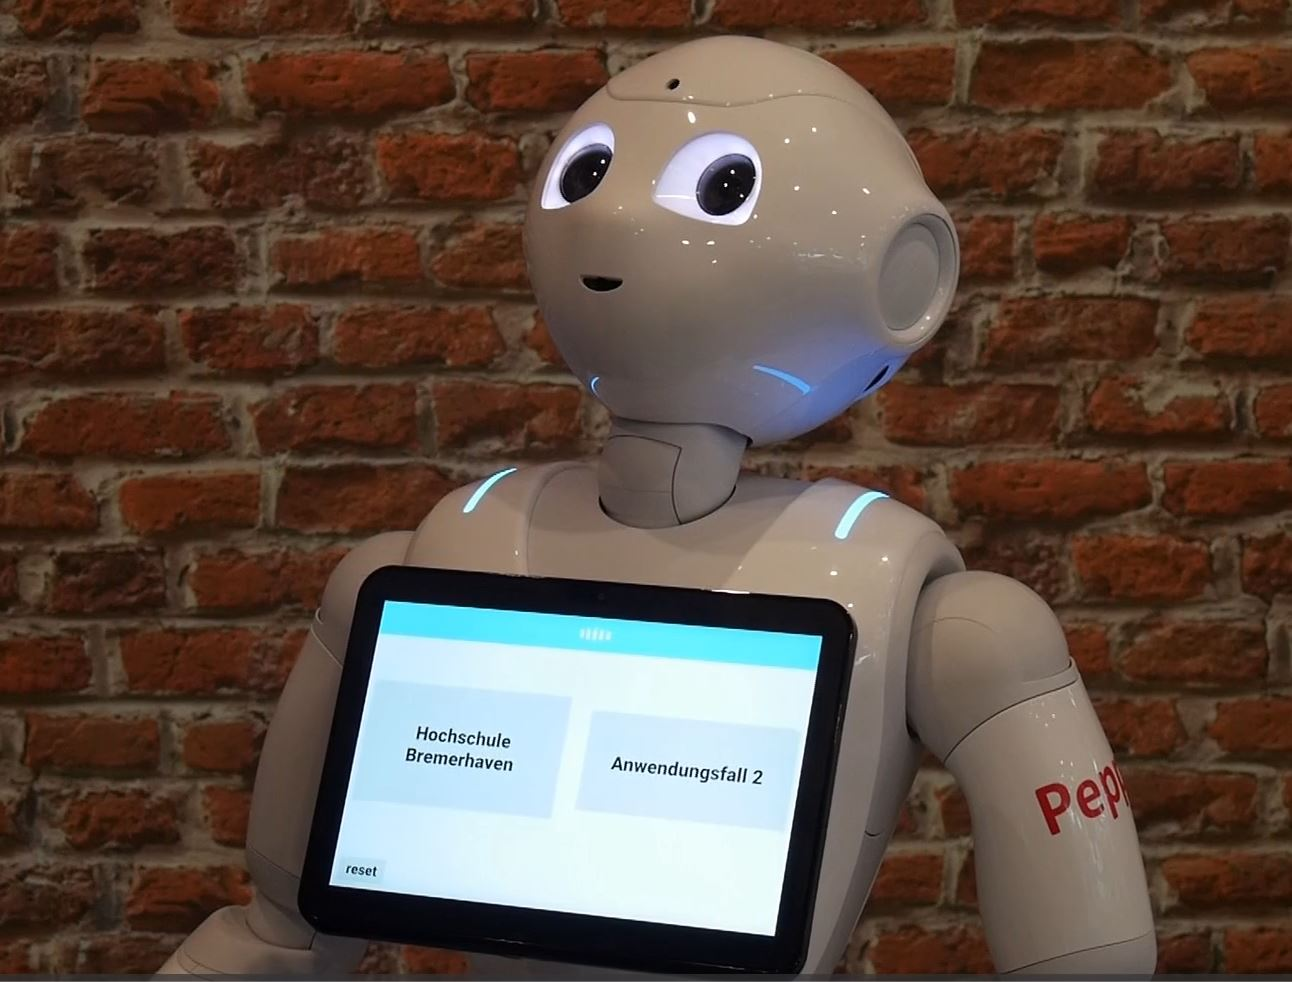
\includegraphics[width=10cm]{Figures/AppChapter/rx1.JPG}
    \caption{Pepper Main Menu}
    \label{fig:Mainmenu}
    \centering
\end{figure}

Eine Applikation, die aus vielen umfangreiche Themen besteht, zieht den größten Nutzen aus der Fragmentfunktion. Themen, die sich stark voneinander unterscheiden, werden somit voneinander getrennt gehalten und die Applikation spart somit auch an Ressourcen.\\

\subsubsection{Chatbot und Topics}

Wie bereits erwähnt, wird der Chatbot in der \verb|onRobotFocusGained| Methode aufgerufen. Sobald Pepper eine Person fokussiert, wird der Chatbot als asynchrone Instanz bereitgestellt. Bei der Initialisierung stellen wir zuerst die Sprache, die Pepper beim Sprechen verwenden soll, auf Deutsch und geben anschließend alle Topic Dateien an, die Pepper verwenden soll. In unserer Applikation verwenden wir hauptsächlich die Topics \verb|background| und \verb|concepts|. Das \verb|concepts| Topic dient als Erweiterung für das \verb|background| Topic, da hier mehrere Wörter zu einem Klasse zusammengefasst werden.\\

\begin{lstlisting}[caption={Konzept - Beispiel}]
concept:(hallo)[hey hallo moin na "guten Tag"]
\end{lstlisting}

Diese können anschließend in dem background Topic wie folgt verwendet werden:\\

\begin{lstlisting}[caption={Topic - Beispiel}]
u:(~hallo {Pepper}) 	Hey, schoen dich zu sehen
\end{lstlisting}

Nun kann Pepper mehrere Variationen von Begrüßungen verstehen.

In den Topics gibt es viele weitere hilfreiche Funktionen, die es zum Beispiel ermöglichen, die aktuelle Uhrzeit oder das Datum als Antwort 
mitzugeben. \\

\begin{lstlisting}[caption={Topic - Datum}]
u:(~welche-uhrzeit) ^currentTime
u:(~datum) Heute ist der ^currentDate
\end{lstlisting}

Es ist ebenfalls möglich, dass Peppers eine zufällige Antwort zu einer bestimmten Frage gibt. Diese kann wie folgt definiert werden:\\

\begin{lstlisting}[caption={Topic - Zufallsantwort}]
    u:([Erzaehl Sag] {mir} {ein} Witz) ^rand[
        "Kommt ein Pferd in die Bar. Fragt der Barkeeper, Hey warum 
        so ein langes Gesicht"
        "Wenn Chuck Norris einen Windows Update macht, akzeptiert 
        Microsoft seine Bedingungen."
        "129 Prozent der Leute uebertreiben voellig"
    ]
\end{lstlisting}

Pepper sucht sich hier eine zufällige Antwort aus und erwidert diese auf die Frage ``Erzähl mir einen Witz''. 

Der größte Vorteil an den Topics ist das Aufrufen einer Methode zu einer bestimmten Frage. 
Hierbei können einzelne Wörter, die Pepper in der Frage erkannt hat, als Variable mitgeben werden aber auch das übergeben einer Variable von 
der Methode zur Antwort ist möglich.\\

\begin{lstlisting}[caption={Topic - Methodenaufruf}]
    u:({was} {gibt{s}} {es} {zu} essen {am} _[~week]) $day=$1 
    ^execute(VariableExecutor, qiVariableMensa, $day) $day gibt 
    es entweder $qiVariableMensa.
\end{lstlisting}

Mit \verb|execute| wird der Methodenaufruf gestartet. Die Methode, die aufgerufen wird, befindet sich in der Klasse \verb|VariableExecutor|.  In dieser Klasse befindet sich eine \verb|runWith| Methode, die automatisch ausgeführt wird, wenn die \verb|execute| Funktion in dem Topic  erreicht wurde. Die einzelnen Argumente in dieser Funktion sind String Parameter, die wir der Methode \verb|runWith| mitgeben. Das Argument \verb|qiVariableMensa| wird dazu verwendet, um mittels \verb|switch case| Befehlen unterscheiden können, welche Frage getriggert wurde. Alle weiteren Argumente dienen als weitere String Parameter, die wir der Methode übergeben wollen. Sobald die Methode erreicht wurde, gibt es die Möglichkeit, die mitgegeben Parameter umzuschreiben und der Antwort in dem Topic wieder zurückzugeben. \verb|getCurrentChatBot().setQiVariable(variableName,'Ich bin jetzt die neue qiVariable');|%das in einem listing?\\

\subsubsection{Webview}

Die Webview ist eine nützliche Funktion von Android Studio, die es erlaubt, ganze Webseiten auf dem Tablet von Pepper abzubilden. Man könnte sie ungefähr mit IFrames von HTML vergleichen. In Android Studio funktioniert die Implementierung ungefähr genau sowie die \verb|setContentView| Funktion, da sie ebenfalls auf dem UI-Thread ausgeführt werden muss. Doch davor müssen noch ein paar wichtige Einstellungen vorgenommen werden, bis diese Funktion implementieren kann. Als Erstes muss die Verbindung mit dem Internet in der \verb|AndroidManifest.xml| erlaubt werden. Wie bereits erwähnt, müssen dafür \verb|permissions| geschrieben werden. \\

\begin{lstlisting}[caption={Internetzugriff erlauben}]
<uses-permission android:name="android.permission.INTERNET" />
<uses-permission android:name="android.permission
.ACCESS_NETWORK_STATE" />
\end{lstlisting}

Nachdem der Internetzugriff in unserer Applikation erlaubt war, ist der nächste Schritt das Erstellen einer Konfigurationsdatei, um die Netzwerksicherheit zu gewähren. Mit dem Befehl: \verb|<base-config cleartextTrafficPermitted="true" />| stellen wir sicher, dass nur Webseiten mit \verb|https| aufgerufen werden dürfen.  %Sollte der Webviewer über einen Klartext-Netzwerkverkehr wie z.B HTTP kommunizieren, könnte dies das Risiko des Abhörens und der Manipulation von Inhalten erhöhen. Standardmäßig ist diese Option auf \verb|false| gesetzt. 
Sollte der Webviewer über einen Klartext-Netzwerkverkehr wie z.B HTTP kommunizieren, könnte dies das Risiko erhöhen, dass bestimmte Inhalte manipuliert oder abgehört werden. Standardmäßig ist diese Option auf \verb|false| gesetzt. 
(Quelle: \cite{webview})

Als Nächstes muss das Layout erstellt werden und eine WebView muss als Komponente mit einer eindeutigen Id hinzugefügt werden. Diese Id kann im Code mithilfe der Funktion \verb|findViewById| rausgesucht und mit einem WebView Objekt initialisiert werden. Wenn die Webseite, die wir 
auf dem Tablet widerspiegeln wollen, Javascript verwendet, müssen wir diese zusätzlich in den Einstellungen der WebView, mittels \verb|webSettings.setJavaScriptEnabled(true)|, erlauben. Mit \verb|web.loadUrl(‘https:...’)| kann anschließend unsere URL von der Webseite, die wir verwenden wollen, in die WebView geladen werden. 

Nun würde sich normalerweise der Standardbrowser des Tablets öffnen, sollte der Anwender in der Webview eine Weiterleitung zu einer anderen Webseite öffnen. Um dies zu verhindern, muss die WebViewClient verändert werden, sodass ein weiterer Webview geöffnet wird, falls dieser Fall eintrifft. Dies kann wie folgt implementiert werden: \\

\begin{lstlisting}[language=Java, caption={Webview Grundgerüst}]
web.setVebViewClient(new Callback())
try{
    ma.runOnUiThread(() -> {
        ma.setContentView(R.layout.webtest);
        WebView web = (WebView) ma.findViewById(R.id.webView);
        WebSettings webSettings = web.getSettings();
        webSettings.setJavaScriptEnabled(true);
        web.setWebViewClient(new Callback());
        web.loadUrl(url);
    });
}catch (Exception e){
    e.printStackTrace();
}

private class Callback extends WebViewClient {
    @Override
    public boolean shouldOverrideKeyEvent(WebView view, KeyEvent event){
        return false;
    }
}
\end{lstlisting}
Wir haben längere Zeit Schwierigkeiten, den WebViewer auf dem Emulator zum Laufen zu bringen. Sobald dieser im Code erreicht wurde, kam eine Fehlermeldung, dass die GPU zu leistungsschwach wäre, um diese Aktion durchzuführen. In der älteren Version von Android Studio hat der WebViewer 
jedoch noch funktioniert. Mit der jetzigen Version ist es zurzeit nicht möglich, die Webview auf dem Emulator auszuführen und muss deshalb auf einen richtigen Pepper getestet werden.\\

\subsubsection{HumanAwareness}

Damit Pepper weiß, wann er einen Anwender fokussieren soll, gibt es die Möglichkeit, auf die \verb|humanAwareness| Funktion zuzugreifen. Diese ist mit den Kameras und Distanzsensoren von Pepper verbunden. Die Kameras von Pepper befinden sich in seinen beiden Augen und sind mit einer Gesichtserkennung ausgestattet. Die \verb|humanAwareness| Funktion bietet nun eine Vielzahl an Einstellungsmöglichkeiten, wann eine Person von Pepper erkannt wird und wann nicht. Es kann zum Beispiel eingestellt werden, ab welcher Distanz eine Person erst erkannt werden soll. Ist die Distanz sehr niedrig eingestellt, wird Pepper nur nach Personen suchen, die sich in seinem nahen Umfeld befinden. Auch die Distanz, ab wann er den Fokus verlieren soll, kann eingestellt werden. Sollte Pepper einen Anwender fokussiert haben, ignoriert er alle weiteren Personen in seinem Umfeld. Mit der \verb|humanAwareness| können auch Gruppen von Menschen erkannt werden und Pepper kann zuordnen, ob es sich um eine Familie handelt oder ein Freundeskreis. Sollte zum Beispiel eine Gruppe aus jungen und älteren Menschen vor Pepper stehen, ordnet Pepper sie zu einer Familie zu.\\

\subsubsection{Personenerkennung}

Peppers Kamera besitzt verschiedene KI basierte Anwendungen, um bestimmte Eigenschaften des Anwenders ermitteln zu können. Dies dient dafür, verschiedene Daten über den Anwender zu sammeln, um daraus zum Beispiel das Nutzerverhalten zu analysieren.

Folgende Daten können über den Anwender gesammelt werden:
\begin{itemize}
    \item Alter
    \item Geschlecht
    \item Emotionen
\end{itemize}

Diese Eigenschaften sind von Softbanks fest vorgegeben und können nicht erweitert werden. Pepper kann anhand der Emotionen erkennen, ob der Anwender glücklich, neutral, genervt oder traurig ist.\\

\subsubsection{No Interaction Timer}

Nachdem Pepper bereits mehrere Interaktionsmöglichkeiten und Ansichten auf seinem Tablet besaß, hatten wir das Problem, dass wir nicht mehr von einem beliebigen View zum Hauptmenü wechseln konnten. Wenn ein Anwender sich zum Beispiel den Mensaplan auf dem Tablet anzeigen lässt, wäre er nicht mehr in das Hauptmenü zurückgekommen. 

Aus diesem Grund haben wir Pepper beigebracht, ins Hauptmenü zu wechseln, sobald der Anwender ``Zurück'' sagt. Nun konnte zu jeder Zeit während des Gesprächs in das Hauptmenü gewechselt werden. Sollte der Anwender jedoch das Gespräch mit Pepper verlassen, während er sich nicht im Hauptmenü befindet, so würde der nächste Anwender die Ansicht sehen, der zuletzt verwendet wurde. 
Um dies zu vermeiden, haben wir eine Klasse geschrieben, welche die View automatisch zurücksetzt.
Sollte über eine vordefinierte Zeit keine Interaktion mit Pepper stattgefunden haben, so wird automatisch zum Hauptmenü gewechselt.